%%%%%%%%%%%%%%%% Relojes Bloom.
\begin{frame}[fragile]{Relojes Bloom:}{Filtro Bloom. Falsos positivos.}
  \justifying
  ¿Será cierto qué todos los elementos para los cuales
  las \textit{hash-funciones} nos regresen valores que en
  el \textit{bloom-filtro}  tienen asigando $1$,
  son valores que han sido introducidos al filtro?
  \begin{figure}
    \centering
    \begin{subfigure}[b]{0.5\textwidth}
      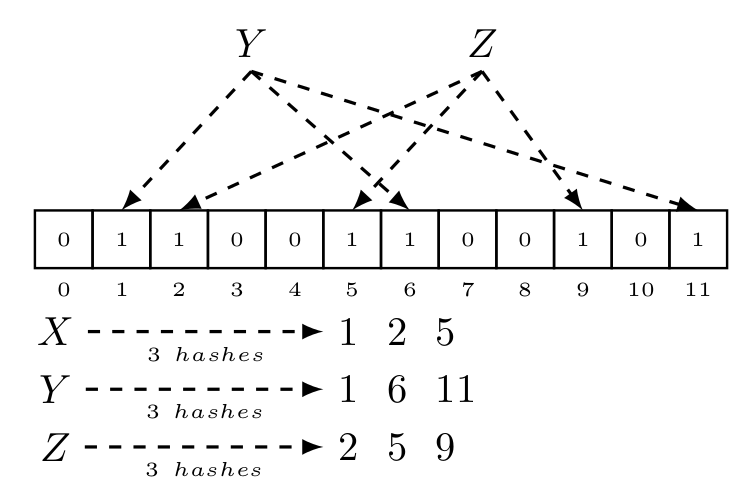
\includegraphics[width=\textwidth]{./Imagenes/FalsosPositivos}
      \caption{Falsos Positivos.}
      \label{fig:Ejemplo de un Falso Positivo.}
    \end{subfigure}
  \end{figure}
  ¿Qué podemos hacer? ...
\end{frame}

